\chapter{Тригонометрические уравнения, отбор корней и неравенства}\label{chap:exam-trigonometric}\markright{Глава 25}
\section{Все решения простейших уравнений}
Все углы измеряем в радианах, а \(k\) в формулах общих решений пробегает \(\mathbb Z\). Одно найденное значение синуса или косинуса обычно соответствует бесконечному множеству углов. Задача на всей прямой требует описать всё это множество.
\begin{definition}\term{Общее решение} (general solution) уравнения — запись всех его корней, например с помощью целого параметра.\end{definition}
\begin{definition}\term{Отбор корней} (selection of roots) оставляет из общего решения только значения, удовлетворяющие дополнительному ограничению.\end{definition}
\begin{definition}\term{Арккотангенс} (arccotangent) \(\operatorname{arcctg}a\) — единственный угол \(\beta\in(0;\pi)\), для которого \(\operatorname{ctg}\beta=a\). При такой договорённости \(\operatorname{arcctg}a=\frac\pi2-\operatorname{arctg}a\).\end{definition}
\begin{theorem}[Четыре общие формулы]
При \(|a|\leq1\), \(\alpha=\arcsin a\), \(\beta=\arccos a\)
\[
\begin{aligned}
\sin x=a&\ \Longleftrightarrow\ x=\alpha+2\pi k\ \text{или}\ x=\pi-\alpha+2\pi k,\\
\cos x=a&\ \Longleftrightarrow\ x=\beta+2\pi k\ \text{или}\ x=-\beta+2\pi k.
\end{aligned}
\]
При \(|a|>1\) оба уравнения решений не имеют. Для любого действительного \(a\)
\[
\begin{aligned}
\operatorname{tg}x=a&\ \Longleftrightarrow\ x=\operatorname{arctg}a+\pi k,\\
\operatorname{ctg}x=a&\ \Longleftrightarrow\ x=\operatorname{arcctg}a+\pi k.
\end{aligned}
\]
\end{theorem}
\begin{proof}Горизонтальная прямая с ординатой \(a\) пересекает единичную окружность в точках с углами \(\alpha\), \(\pi-\alpha\) по модулю \(2\pi\). Вертикальная прямая с абсциссой \(a\) даёт углы \(\beta,-\beta\). При \(a=\pm1\) две точки сливаются, и две серии описывают одно множество; вне диапазона \([-1;1]\) пересечений нет. Тангенс на каждой ветви \((-\frac\pi2+\pi k;\frac\pi2+\pi k)\) строго возрастает от сколь угодно больших отрицательных значений до положительных, а котангенс на \((\pi k;\pi+\pi k)\) строго убывает в обратном направлении. Периодичность переносит единственный корень основной ветви на все остальные. Формула для арккотангенса следует из \(\operatorname{ctg}(\frac\pi2-t)=\operatorname{tg}t\) при \(t\in(-\frac\pi2;\frac\pi2)\).\end{proof}
Для синуса можно использовать и одну запись \(x=(-1)^k\alpha+\pi k\). При \(a=0\) она даёт \(x=\pi k\), при \(a=1\) — \(x=\frac\pi2+2\pi k\) после удаления повторов. Для косинуса при \(a=1\) имеем \(x=2\pi k\), при \(a=-1\) — \(x=\pi+2\pi k\).
\par\addvspace{2pt}\begin{lrbox}{\CatFlowBox}\begin{minipage}[t]{\linewidth}
\setlength{\parskip}{2pt}\setlength{\columnsep}{4.5mm}\setlength{\intextsep}{0pt}
\begin{wrapfigure}[11]{r}{54mm}

\includegraphics[width=54mm,height=58mm,keepaspectratio]{images/unique/art-230.png}
\label{catflow:230}
\end{wrapfigure}
Единичная окружность помогает увидеть полноту общего решения. Горизонтальная или вертикальная прямая сначала даёт точки одного оборота, а затем к каждому найденному углу прибавляют целое число полных оборотов. Для тангенса и котангенса достаточно полуоборотов, поскольку одновременно меняются знаки числителя и знаменателя. Однако период функции и расстояние между соседними корнями конкретного уравнения могут различаться. Например, нули синуса встречаются через полоборота, хотя сам синус имеет больший период. Поэтому удобно проверять запись в двух направлениях: каждый указанный угол должен подходить, а каждый возможный угол должен попасть в одну из серий. Повторы серий допустимы, но в конечном списке корней одинаковые значения записывают один раз.
\par\WFclear\end{minipage}\end{lrbox}%
\ifdim\dimexpr\ht\CatFlowBox+\dp\CatFlowBox\relax<58mm\dp\CatFlowBox=\dimexpr58mm-\ht\CatFlowBox\relax\fi%
\noindent\usebox{\CatFlowBox}\par\addvspace{2pt}
\begin{example}Решим \(\operatorname{tg}(2x-\frac\pi6)=\sqrt3\). Сначала \(2x-\frac\pi6=\frac\pi3+\pi k\), затем \(x=\frac\pi4+\frac\pi2k\). Эти значения не попадают в запрещённые точки тангенса, поскольку его аргумент равен \(\frac\pi3\) по модулю \(\pi\).\end{example}

\section{Периодичность и отбор на промежутке}
Для \(\sin(mx+b)\), \(\cos(mx+b)\), где \(m\ne0\), наименьший положительный период равен \(\frac{2\pi}{|m|}\); для тангенса и котангенса — \(\frac{\pi}{|m|}\). В уравнении сначала находят все значения аргумента, затем решают полученные линейные равенства относительно \(x\). Если \(m=0\), выражение постоянно, и случай рассматривают отдельно.
\begin{theorem}[Отбор целого параметра]
Пусть одна серия корней записана как \(x=c+Tk\), где \(T>0\). На отрезке \([L;U]\) ей отвечают ровно целые числа
\[
\frac{L-c}{T}\leq k\leq\frac{U-c}{T}.
\]
Для открытых концов соответствующий знак также делают строгим.
\end{theorem}
\par\addvspace{2pt}\begin{lrbox}{\CatFlowBox}\begin{minipage}[t]{\linewidth}
\setlength{\parskip}{2pt}\setlength{\columnsep}{4.5mm}\setlength{\intextsep}{0pt}
\begin{wrapfigure}[12]{l}{54mm}

\includegraphics[width=54mm,height=58mm,keepaspectratio]{images/unique/art-233.png}
\label{catflow:233}
\end{wrapfigure}
\textit{Доказательство.} Двойное неравенство получается подстановкой \(L\leq c+Tk\leq U\), вычитанием \(c\) и делением на положительное \(T\). Все действия обратимы.\hfill\(\blacksquare\)
\par\WFclear\end{minipage}\end{lrbox}%
\ifdim\dimexpr\ht\CatFlowBox+\dp\CatFlowBox\relax<58mm\dp\CatFlowBox=\dimexpr58mm-\ht\CatFlowBox\relax\fi%
\noindent\usebox{\CatFlowBox}\par\addvspace{2pt}

\begin{example}Найдём корни \(\cos2x=0\) на \([-\pi;\pi]\). Общее решение \(x=\frac\pi4+\frac\pi2k\). Отбор даёт \(-\frac52\leq k\leq\frac32\), поэтому \(k=-2,-1,0,1\). Ответ: \(-\frac{3\pi}4,-\frac\pi4,\frac\pi4,\frac{3\pi}4\).\end{example}

\section{Квадратные и однородные уравнения}
Замена \(t=\sin x\) или \(t=\cos x\) требует \(-1\leq t\leq1\). После решения квадратного уравнения для каждого допустимого \(t\) записывают все углы. Для замены \(t=\operatorname{tg}x\) допустимы все действительные \(t\), но исходный тангенс должен быть определён.
\begin{example}В \(2\sin^2x+\sin x-1=0\) получаем \((2t-1)(t+1)=0\), то есть \(t=\frac12\) или \(t=-1\). Общее решение: \(x=\frac\pi6+2\pi k\), \(x=\frac{5\pi}6+2\pi k\) или \(x=-\frac\pi2+2\pi k\). Оба значения \(t\) находятся в диапазоне синуса.\end{example}
\begin{definition}\term{Однородное тригонометрическое уравнение второй степени} (homogeneous trigonometric equation of degree two) имеет вид \(A\sin^2x+B\sin x\cos x+C\cos^2x=0\), где \(A,B,C\) — постоянные.\end{definition}
\begin{theorem}[Сведение однородного уравнения к квадратному]
В указанном уравнении значения с \(\cos x=0\) являются корнями ровно при \(A=0\). Для остальных значений деление на \(\cos^2x\) равносильно и даёт \(At^2+Bt+C=0\), где \(t=\operatorname{tg}x\).
\end{theorem}
\begin{proof}При \(\cos x=0\) имеем \(\sin^2x=1\), поэтому левая часть равна \(A\). При \(\cos x\ne0\) делитель положителен и ненулевой; деление даёт нужный многочлен. Каждое его действительное значение \(t\) возвращается к серии \(x=\operatorname{arctg}t+\pi k\). Если многочлен тождественно нулевой, подходят все значения с \(\cos x\ne0\), вместе с уже разобранными случаями.\end{proof}
\begin{example}В \(2\sin^2x-3\sin x\cos x+\cos^2x=0\) точки \(\cos x=0\) не подходят. После деления получаем \((2t-1)(t-1)=0\). Поэтому \(x=\operatorname{arctg}\frac12+\pi k\) или \(x=\frac\pi4+\pi k\).\end{example}
\par\addvspace{2pt}\begin{lrbox}{\CatFlowBox}\begin{minipage}[t]{\linewidth}
\setlength{\parskip}{2pt}\setlength{\columnsep}{4.5mm}\setlength{\intextsep}{0pt}
\begin{wrapfigure}[13]{l}{54mm}
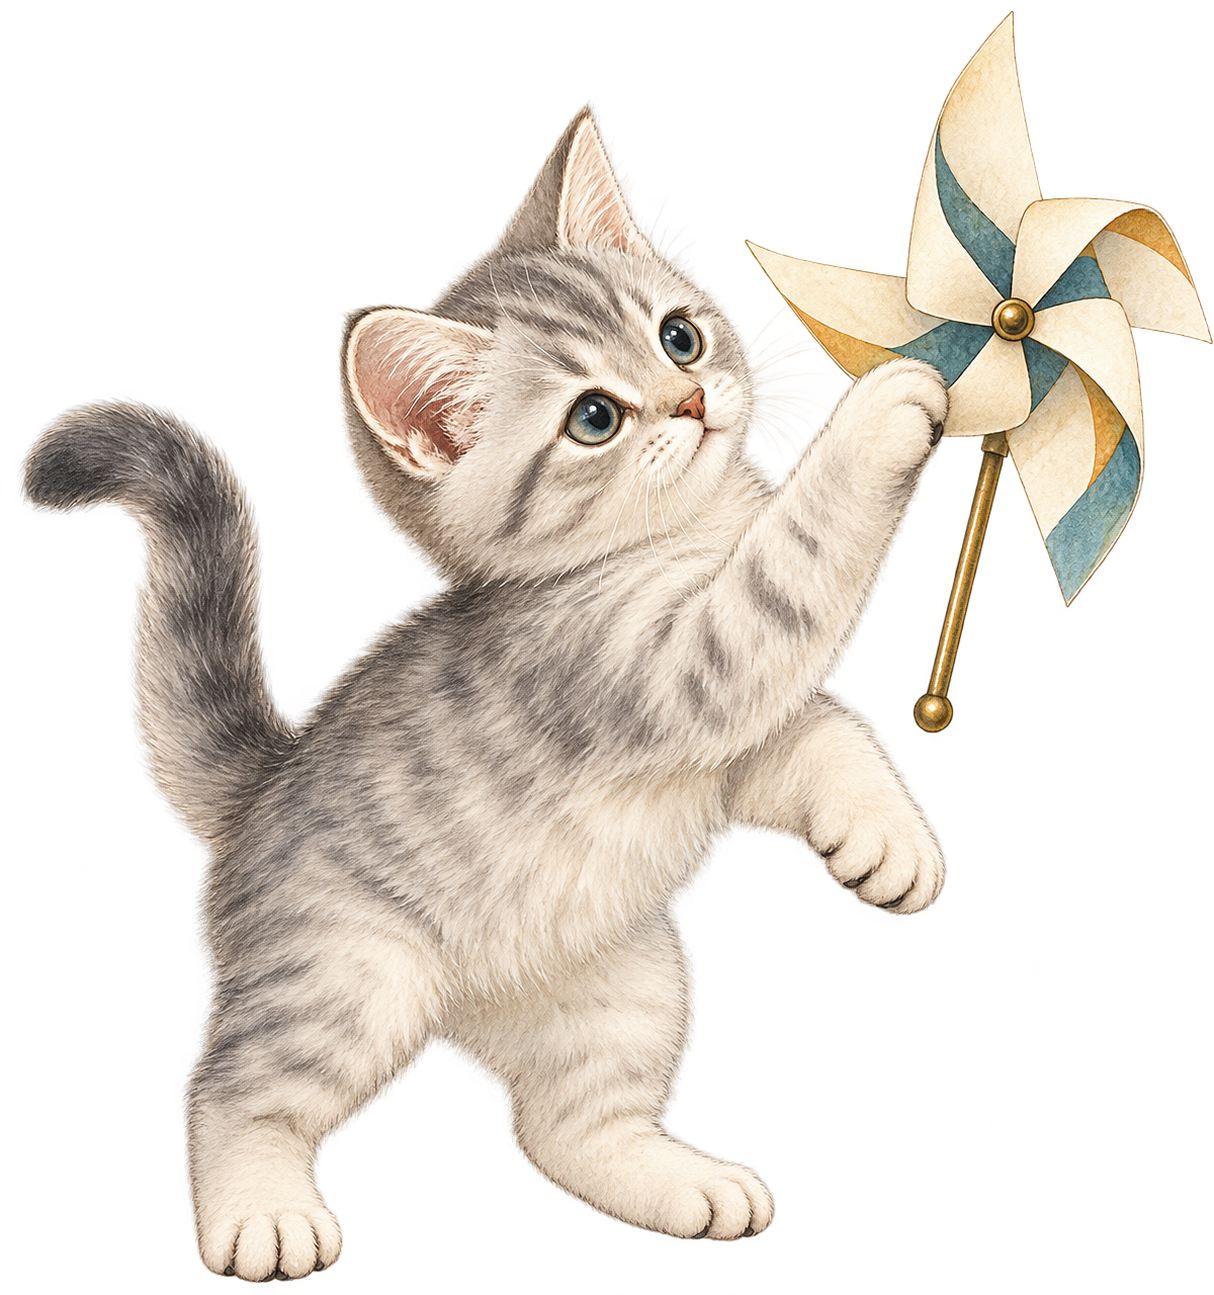
\includegraphics[width=54mm,height=58mm,keepaspectratio]{images/unique/art-231.png}
\label{catflow:231}
\end{wrapfigure}
Перед делением на синус или косинус нужно проверить их нули. В тригонометрических задачах эта привычка сохраняет целые серии решений, которые иначе легко потерять одним действием. Если уравнение уже содержит дробь, запреты знаменателя выписывают до умножения на него. При факторизации нулю может равняться любой множитель, поэтому решают совокупность соответствующих уравнений. При замене на синус или косинус проверяют диапазон нового неизвестного, а затем возвращаются ко всем углам, дающим допустимое значение. Каждое из этих действий имеет отдельную логическую роль. Сначала мы сохраняем область определения, затем находим возможные значения функции и только после этого описываем аргументы. Смешение этих этапов часто приводит к неполному ответу.
\par\WFclear\end{minipage}\end{lrbox}%
\ifdim\dimexpr\ht\CatFlowBox+\dp\CatFlowBox\relax<61mm\dp\CatFlowBox=\dimexpr61mm-\ht\CatFlowBox\relax\fi%
\noindent\usebox{\CatFlowBox}\par\addvspace{2pt}
\section{Сумма в произведение и вспомогательный угол}
\begin{theorem}[Формулы суммы и разности]
Для любых действительных \(u,v\)
\[
\begin{aligned}
\sin u+\sin v&=2\sin\frac{u+v}2\cos\frac{u-v}2,\\
\sin u-\sin v&=2\cos\frac{u+v}2\sin\frac{u-v}2,\\
\cos u+\cos v&=2\cos\frac{u+v}2\cos\frac{u-v}2,\\
\cos u-\cos v&=-2\sin\frac{u+v}2\sin\frac{u-v}2.
\end{aligned}
\]
\end{theorem}
\begin{proof}Положим \(s=\frac{u+v}2\), \(t=\frac{u-v}2\), так что \(u=s+t,v=s-t\). Складывая и вычитая формулы \(\sin(s\pm t)=\sin s\cos t\pm\cos s\sin t\), получаем первые две строки. Формулы \(\cos(s\pm t)=\cos s\cos t\mp\sin s\sin t\) дают последние две.\end{proof}
Если \(R=\sqrt{a^2+b^2}>0\), выбирают угол \(\varphi\) так, что \(\cos\varphi=\frac aR\), \(\sin\varphi=\frac bR\). Формула сложения даёт \(a\sin x+b\cos x=R\sin(x+\varphi)\). Такой угол существует, поскольку сумма квадратов выбранных координат равна единице. Если \(a=b=0\), выражение постоянно равно нулю и делить на \(R\) нельзя.
\begin{example}Равенство \(\sin x+\cos x=1\) превращается в \(\sqrt2\sin(x+\frac\pi4)=1\). Поэтому \(x+\frac\pi4=\frac\pi4+2\pi k\) или \(x+\frac\pi4=\frac{3\pi}4+2\pi k\). Ответ: \(x=2\pi k\) или \(x=\frac\pi2+2\pi k\).\end{example}

\section{Тригонометрические неравенства}
\begin{theorem}[Основные промежутки решений]
Пусть \(-1<a<1\), \(\alpha=\arcsin a\), \(\beta=\arccos a\). Тогда множества решений являются объединениями по \(k\in\mathbb Z\) следующих промежутков:
\[
\begin{aligned}
\sin x\geq a &: [\alpha+2\pi k;\pi-\alpha+2\pi k],\\
\sin x\leq a &: [\pi-\alpha+2\pi k;2\pi+\alpha+2\pi k],\\
\cos x\geq a &: [-\beta+2\pi k;\beta+2\pi k],\\
\cos x\leq a &: [\beta+2\pi k;2\pi-\beta+2\pi k].
\end{aligned}
\]
Для любого \(a\in\mathbb R\), \(\gamma=\operatorname{arctg}a\), \(\delta=\operatorname{arcctg}a\) имеем
\[
\begin{aligned}
\operatorname{tg}x\geq a &: [\gamma+\pi k;\frac\pi2+\pi k),\\
\operatorname{tg}x\leq a &: (-\frac\pi2+\pi k;\gamma+\pi k],\\
\operatorname{ctg}x\geq a &: (\pi k;\delta+\pi k],\\
\operatorname{ctg}x\leq a &: [\delta+\pi k;\pi+\pi k).
\end{aligned}
\]
\end{theorem}
\begin{proof}На окружности знак сравнения синуса с \(a\) определяется положением выше или ниже горизонтальной прямой; косинуса — правее или левее вертикальной. Граничные углы взяты из общих формул уравнений, а подходящие дуги дают записанные промежутки. Для тангенса используем возрастание на каждой ветви, для котангенса — убывание. Концы ветвей, где функция не определена, остаются открытыми.\end{proof}
При строгом сравнении исключают точки равенства. При \(a=\pm1\) отдельно используют диапазон синуса или косинуса и их точки максимума и минимума: например, \(\sin x\geq1\) имеет только корни \(\frac\pi2+2\pi k\), а \(\sin x>-1\) исключает ровно \(-\frac\pi2+2\pi k\). При \(a>1\) или \(a<-1\) сравнение решается непосредственно по диапазону \([-1;1]\).
\par\addvspace{2pt}\begin{lrbox}{\CatFlowBox}\begin{minipage}[t]{\linewidth}
\setlength{\parskip}{2pt}\setlength{\columnsep}{4.5mm}\setlength{\intextsep}{0pt}
\begin{wrapfigure}[9]{r}{54mm}

\includegraphics[width=54mm,height=58mm,keepaspectratio]{images/unique/art-232.png}
\label{catflow:232}
\end{wrapfigure}
Дуга решения на окружности задаёт промежутки на прямой после добавления полных периодов. Строгость знака определяет, включены ли граничные углы, а область определения отдельно исключает разрывы тангенса и котангенса. В системе нужно пересечь найденные множества. Часто удобнее сначала выполнить пересечение на одном общем периоде и затем перенести результат, но сначала необходимо убедиться, что выбранный сдвиг является периодом каждого условия. При отборе на заданном отрезке периодический ответ пересекают ещё и с этим отрезком. Положительные и отрицательные границы проверяют одинаково внимательно: округление углов или целого параметра способно добавить лишний корень. Точные дроби от числа пи сохраняют такую проверку простой и наглядной.
\par\WFclear\end{minipage}\end{lrbox}%
\ifdim\dimexpr\ht\CatFlowBox+\dp\CatFlowBox\relax<58mm\dp\CatFlowBox=\dimexpr58mm-\ht\CatFlowBox\relax\fi%
\noindent\usebox{\CatFlowBox}\par\addvspace{2pt}
\begin{example}Решим систему \(\sin x\geq0\), \(\cos x\leq0\). На одном обороте первая часть допускает верхнюю полуокружность, вторая — левую. Их пересечение — вторая четверть вместе с концами: \([\frac\pi2;\pi]\). Общий ответ: \(x\in[\frac\pi2+2\pi k;\pi+2\pi k]\), \(k\in\mathbb Z\).\end{example}

\relax

\Needspace{7\baselineskip}\section*{Задачи}
\begingroup\setlength{\parskip}{1pt}
\noindent\begin{minipage}[t]{\linewidth}\textbf{25.1.} Реши на всей прямой \(\sin x=-\dfrac12\).\par\end{minipage}\par
\noindent\begin{minipage}[t]{\linewidth}\textbf{25.2.} Реши \(\cos x=-\dfrac{\sqrt2}2\).\par\end{minipage}\par
\noindent\begin{minipage}[t]{\linewidth}\textbf{25.3.} Реши \(\operatorname{tg}(2x-\dfrac\pi6)=\sqrt3\).\par\end{minipage}\par
\noindent\begin{minipage}[t]{\linewidth}\textbf{25.4.} Реши \(\operatorname{ctg}(3x)=-1\).\par\end{minipage}\par
\noindent\begin{minipage}[t]{\linewidth}\textbf{25.5.} Реши \(\sin x=2\).\par\end{minipage}\par
\par\addvspace{2pt}\begin{lrbox}{\CatFlowBox}\begin{minipage}[t]{\linewidth}
\setlength{\parskip}{2pt}\setlength{\columnsep}{4.5mm}\setlength{\intextsep}{0pt}
\begin{wrapfigure}[13]{r}{54mm}

\includegraphics[width=54mm,height=58mm,keepaspectratio]{images/unique/art-234.png}
\label{catflow:234}
\end{wrapfigure}
\textbf{25.6.} Реши \(\cos2x=1\).\par

\textbf{25.7.} Реши \(\sin3x=0\).\par

\textbf{25.8.} Реши \(\sin(2x+\dfrac\pi3)=1\).\par

\textbf{25.9.} Реши \(\sin x=\sin\dfrac\pi7\).\par
\par\WFclear\end{minipage}\end{lrbox}%
\ifdim\dimexpr\ht\CatFlowBox+\dp\CatFlowBox\relax<61mm\dp\CatFlowBox=\dimexpr61mm-\ht\CatFlowBox\relax\fi%
\noindent\usebox{\CatFlowBox}\par\addvspace{2pt}

\noindent\begin{minipage}[t]{\linewidth}\textbf{25.10.}\starmark{} Реши \(\cos x=\cos2x\).\par\end{minipage}\par
\noindent\begin{minipage}[t]{\linewidth}\textbf{25.11.}\starmark{} Реши \(\sin2x=\sin x\).\par\end{minipage}\par
\noindent\begin{minipage}[t]{\linewidth}\textbf{25.12.} Реши \(2\cos^2x-3\cos x+1=0\).\par\end{minipage}\par
\noindent\begin{minipage}[t]{\linewidth}\textbf{25.13.} Реши \(2\sin^2x+\sin x-1=0\).\par\end{minipage}\par
\noindent\begin{minipage}[t]{\linewidth}\textbf{25.14.} Реши \(\sin x+\cos x=1\).\par\end{minipage}\par
\noindent\begin{minipage}[t]{\linewidth}\textbf{25.15.}\starmark{} Реши \(2\sin^2x-3\sin x\cos x+\cos^2x=0\).\par\end{minipage}\par
\noindent\begin{minipage}[t]{\linewidth}\textbf{25.16.} Реши \(\sin^2x-\sin x\cos x=0\).\par\end{minipage}\par
\noindent\begin{minipage}[t]{\linewidth}\textbf{25.17.}\starmark{} Реши \(\sin3x+\sin x=0\).\par\end{minipage}\par
\noindent\begin{minipage}[t]{\linewidth}\textbf{25.18.}\starmark{} Реши \(\cos3x-\cos x=0\).\par\end{minipage}\par
\noindent\begin{minipage}[t]{\linewidth}\textbf{25.19.}\starmark{} Реши \(\dfrac{\sin2x}{\cos x}=1\).\par\end{minipage}\par
\noindent\begin{minipage}[t]{\linewidth}\textbf{25.20.}\starmark{} Реши \(\operatorname{tg}x+\operatorname{ctg}x=2\).\par\end{minipage}\par
\noindent\begin{minipage}[t]{\linewidth}\textbf{25.21.} Отбери корни \(\sin x=-\dfrac{\sqrt3}2\) на \([-2\pi;0]\).\par\end{minipage}\par
\noindent\begin{minipage}[t]{\linewidth}\textbf{25.22.} Отбери корни \(\cos2x=0\) на \([-\pi;\pi]\).\par\end{minipage}\par
\noindent\begin{minipage}[t]{\linewidth}\textbf{25.23.} Реши \(\sin x\geq\dfrac12\).\par\end{minipage}\par
\noindent\begin{minipage}[t]{\linewidth}\textbf{25.24.} Реши \(\cos x<-\dfrac12\).\par\end{minipage}\par
\noindent\begin{minipage}[t]{\linewidth}\textbf{25.25.} Реши \(\operatorname{tg}x\leq1\).\par\end{minipage}\par
\noindent\begin{minipage}[t]{\linewidth}\textbf{25.26.} Реши \(\operatorname{ctg}x>0\).\par\end{minipage}\par
\noindent\begin{minipage}[t]{\linewidth}\textbf{25.27.} Реши \(\sin2x>0\) на \([0;2\pi]\).\par\end{minipage}\par
\noindent\begin{minipage}[t]{\linewidth}\textbf{25.28.} Реши систему \(\sin x\geq0\), \(\cos x\leq0\).\par\end{minipage}\par
\noindent\begin{minipage}[t]{\linewidth}\textbf{25.29.}\starmark{} Реши \(\sin^2x\leq\dfrac14\).\par\end{minipage}\par
\noindent\begin{minipage}[t]{\linewidth}\textbf{25.30.}\starmark{} Реши \(\cos2x-\cos x=0\) и отбери корни на \([-2\pi;0]\).\par\end{minipage}\par
\noindent\begin{minipage}[t]{\linewidth}\textbf{25.31.}\starmark{} Найди наименьший положительный период \(f(x)=\sin^2(3x)\).\par\end{minipage}\par
\par\Needspace{12\baselineskip}\section*{Олимпиадные задачи}
\par\addvspace{2pt}\begin{lrbox}{\CatFlowBox}\begin{minipage}[t]{\linewidth}
\setlength{\parskip}{2pt}\setlength{\columnsep}{4.5mm}\setlength{\intextsep}{0pt}
\begin{wrapfigure}[13]{r}{54mm}

\includegraphics[width=54mm,height=58mm,keepaspectratio]{images/unique/art-308.png}
\label{catflow:308}
\end{wrapfigure}
\textbf{25.32.}\starmark{} {\small\itshape\href{https://www.imo-official.org/assets/documents/problems/1961/1961_eng.pdf}{IMO, 1961, № 3}; перевод.}\par Реши \(\cos^n x-\sin^n x=1\) для произвольного натурального \(n\).\par

\textbf{25.33.}\starmark{} {\small\itshape\href{https://www.imo-official.org/assets/documents/problems/1962/1962_eng.pdf}{IMO, 1962, № 4}; перевод.}\par Реши \(\cos^2x+\cos^2(2x)+\cos^2(3x)=1\).\par
\par\WFclear\end{minipage}\end{lrbox}%
\ifdim\dimexpr\ht\CatFlowBox+\dp\CatFlowBox\relax<61mm\dp\CatFlowBox=\dimexpr61mm-\ht\CatFlowBox\relax\fi%
\noindent\usebox{\CatFlowBox}\par\addvspace{2pt}

\endgroup
